%% abstrakte simplizialkomplexe

\section{Abstrakte Simplizialkomplexe}

Für topologische Anwendung ist der $\R^J$ in vielen Fällen zu konkret
und unnötiger gedanklicher Balast. Deshalb sollte man die
Simplizialkomplexe unabhängig vom euklidischen Raum definieren. Diese
abstrakten Simplizialkomplexe werden in diesem Abschnitt
behandelt. Die zunächst stark erscheinende Vereinfachung, stellt sich
als eine äquivalente Darstellung zu den geometrischen Komplexen
heraus.

\begin{Def}
  Eine beliebige, nichtleere Menge $\Delta$ heißt \textbf{abstrakter
    Simplizialkomplex} oder auch nur abstrakter Komplex, falls mit
  jedem Element aus $\Delta$ auch jede Teilmenge aus diesem Element in
  $\Delta$ enthalten ist und jedes Element eine endliche
  Menge ist. Oder in Formeln geschrieben
%  \setcounter{equation}{(*)}
\renewcommand*{\theequation}{\textbullet}
  \begin{gather}
    \sigma \in \Delta \text{ und }  \tau \subset \sigma
    \Rightarrow \tau \in \Delta
  \end{gather}
  Für einen abstrakten Komplex werden folgende Begriffe benötigt
  \begin{enumerate}[({A}1)]
% dimension, seite, knoten, unterkomplex, simpliziale abbildung, isomorphie
  \item Ein Element des Komplexes heißt \textbf{Seite}. Die Teilmenge aller
    Seiten der Mächtigkeit kleiner gleich $k$ heißt das \textbf{$k$-Skelett},
    insbesondere für $k=1$ ist dies die \textbf{Knotenmenge}.
  \item Die \textbf{Dimension} des Komplexes ist das Supremum über die
    Mächtigkeit der Seiten von $\Delta$.
  \item Eine Teilmenge vom Komplex die (\textbullet) erfüllt, heißt
    \textbf{Unterkomplex}.
  \item Eine Abbildung zwischen den Knotenmenge zweier abstrakten
    Komplexe heißt \textbf{simpliziale Abbildung}, falls Seiten auf
    Seiten abgebildet werden.
  \item Zwei abstrakte Komplexe heißen \textbf{isomorph}, falls es eine
    bijektive simpliziale Abbildung gibt, deren Inverses auch
    simplizial ist.
  \item Sei $\Delta$ ein geometrischer Komplex so bezeichnet die Menge
    \begin{gather*}
      \set{ \sset{a_0 \ldots a_n} \subset \Delta^{(0)} }{ a_0 \ldots
        a_n \in \Delta}
    \end{gather*}
    das \textbf{Knotenschema} von $\Delta$.
  \item Ist ein abstrakter Komplex $\Delta$ isomorph zum Knotenschema
    eine geometrischen Komplexes $\Delta'$, so nennen wir $\Delta'$
    eine \textbf{geometrische Realisierung} von $\Delta$.
  \end{enumerate}
\end{Def}

\begin{Bsp}
  \begin{enumerate}[\textbullet]
  \item Für einen geometrischen Komplex $\sigma$ ist die Menge all
    seiner Seiten ein abstrakter Simplizalkomplex und das Knotenschema
    wird auf triviale Art und Weise geometrisch durch $\sigma$
    realisiert.
  \item Die Menge $\Delta = \sset{%
      \sset{a,b},\sset{a,c},%
      \sset{b,c},\sset{a},\sset{b},\sset{c},\emptyset}$ ist ein Beispiel und 
    seine geometrische Realisierung sieht wie folgt aus
    \begin{center}
      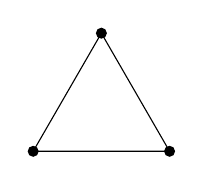
\begin{tikzpicture}
        \draw [thin] (90:1) to (210:1) to (330:1) to (90:1);
        \foreach \foo in {90,210,330}
        \fill (\foo:1) circle[radius=0.07cm];
      \end{tikzpicture}
    \end{center}

  \item Betrachte die Menge
    $\set{ \sset{i,i+1} , \sset{i} }{ i \in \Z} \cup \sset{\emptyset}$
    dann ist der Polyeder zu einer geometrischen Realisierung
    homöomorph zu $\R$

  \item Für eine beliebige Menge ist die Potenzmenge ohne die leere
    Menge stets ein abstrakter Simplizialkomplex
  \item Die von-Neumann Zahlen liefern einen nicht endlichen
    abstrakten Komplex.  Diese Menge erhält man wie folgt, setze
    $V_0 \coloneqq \emptyset$ und
    $V_{n+1} \coloneqq \sset{V_n} \cup \V_n$, dann ist der Komplex
    $V \coloneqq \bigcup\limits_{n \geq 0} V_n$ nicht endlich.
  \item Ein ungerichteter Graph $G=(V,K)$ mit $V$ die Eckmenge und $K$
    die Kanten ist ein abstrakter Simplizialkomplex
  \item Ein Knotenschema von einem geometrisch Komplex ist ein
    abstrakter Komplex (siehe unten)
  \end{enumerate}
\end{Bsp}

% TODO: zeige das für ein element aus \bigcup K ein eindeutiges
% Element aus K existiert so dass das element aus \Int dieses element
% ist

Der Zusammenhang zwischen geometrischen und abstrakten Komplexen ergibt sich 
aus der folgenden Definition.

\begin{Def}[Knotenschema]
\end{Def}

\begin{Bsp}
  foo
  % TODO: füge ein bild von einen geo komplex ein, aus dem das
  % knotenschema extrahiert wird
\end{Bsp}

\begin{Satz}
  Es gelten folgende Aussagen
  \begin{enumerate}[(1)]
  \item Für jeden abstrakten Komplex existiert ein geometrischer
    Komplex dessen Knotenschema (abstrakt) isomorph zu diesem Komplex
    ist.
  \item Zwei geometrisch Komplexe sind (linear) isomorph, genau dann
    wenn die entsprechenden Knotenschemata (abstrakt) isomorph sind.
  \end{enumerate}
  \begin{proof}
%TODO: noch zu beweisen
    foo
  \end{proof}
\end{Satz}

% todo: topologie --literatur/archiv seite 333ff

% erkläre das labeln von triangulierungen, bzw
% geometrischen,abstrakten simplizialkomplexen

\begin{Bem}[Label,Abwicklung]
  Da im weiteren Verlauf des Seminars meist nicht zweidimensionale
  Triangulierungen angegeben und benötigt werden, ist es notwendig
  eine vereinfachte Darstellung dieser höher dimensionalen Objekte
  abzugeben. Hierzu wird das Labeln von Triangulierungen angegeben.

  Betrachte zunächst für die Idee des Verfahrens den Tetraeder und
  seine standard Abwicklung im Zweidimensionalen.
  % zeichne dreidim tetraeder, und eine zweidim abwicklung, tikz
  Bei der Abwicklung werden die $0$-Simplexe fortlaufend alphabetisch
  nummeriert. Bei Knoten die in der ursprünglichen Dimension
  zusammenfallen wird das gleiche Label verwendet.

%TODO: auch für unendlich dimensionale abwicklung
  Die Formalisierung der obigen Idee wird durch die Angabe eines
  abstrakten Komplexes gegeben, dessen geometrische Realisierung dem
  geometrischen Komplex entspricht. Sei $\Delta$ ein endlich
  dimensionaler geometrischer Komplex gegeben. Dann ist die Abwicklung
  durch einen zweidimensionalen geometrischen Komplex $\Delta'$ und
  eine surjektive Abbildung $f: \Delta \rightarrow \Delta'$ gegeben.

%TODO: weiter ausführen

\end{Bem}

% TODO: label und zweidim abwicklungen vom torus, zylinder, kugel und kleinsche flasche

%einfache beispiele

\begin{Bsp}
  Es werden nun Triangulierungen von für Kugel, Zylinder, Torus angegeben.
  Wobei auch die nicht Eindeutigkeit von Triangulierungen anhand des Torus
  aufgezeigt werden.
\end{Bsp}

\begin{Bsp}[Triangulation]
%TODO: beweise folgende triangulierengen \S^2 \simeq \gr{(\Delta^3)^{(2)}}, behauptung diese aussage gilt für allgemeines n, also \S^n \simeq \gr{(\Delta^{n+1})^{(n)}}
\end{Bsp}





% abzählbare mengen können nur durch 0-simplexe trianguliert werden



%Begriffe:
%geometrisch unabhängig, und linear unabhängig vergleichen gegenüberstellen
% simplex, geometrischer simplizialkomplex, abstrakter simplizialkomplex 


% n-ebene, menge von punkten, aufgespannt durch geo.unab system mit konvexkombinationen
% die faktoren sind eindeutig bestimmt

%affine transformation: x -> Ax+b

%geo.unab systeme werden durch affine transformationen auf geo.unab systeme abgebildet

% n simplex

% baryzentrische koordinaten

% ist die leere menge eine simplizial?

% ein simplex ist genau die konvexe hülle von einer endlichen teilmenge vom \R^N

% eine seite eines simplex ist ein teilsimplex der dimension d

% anzahl der d teilsimplexe ist binomial_koeff(n+1,d+1), für einen n dim simplex
% klar wähle aus den n+1 punkten d+1 stück aus

% verwende das schläfli symbol zur beschreibung der umgebung eines
% punktes aus einem simplex für triangulierungen werden nur 2fache
% schläflisymbole benötigt, also {p,q}, da bei der triangulierung nur
% \laplace^2 simplexe verwendet werden, vereinfacht sich das symbol
% auf die form {3,q}. gebe nun zu jedem punkt auf der
% mannigfaltigkeit, also den 0 dimensionalen simplexen, die anzahl der
% angrenzenden dreiecker/laplace^2 simplexe an


% schreibe in die appendix ein eigenen anhang nur mit getikzten beispielen
% die komplette pflasterung von \R^2 oder allgemein die füllung des \R^n mit \laplace^n
% verschiedene triangulierungen

% zeige nicht-kompakte teilmengen vom \R^n sind nicht triangulierbar,
% einfachstes bsp (0,1), einfach das geometrische realisierungen stets
% kompakte mengen sind, somit kann es keinen homöomorphismus geben


%%% Local Variables:
%%% mode: latex
%%% TeX-master: "main"
%%% End: